% File 'template.tex'

\documentclass[12pt]{report}

\usepackage{url}
\usepackage[numbers,sort]{natbib}
% Removed the dvips option
\usepackage{graphicx}
\usepackage{amsmath}
\usepackage{amssymb}
\usepackage{algorithm}
\usepackage{algorithmic}

% If there are any other \usepackage commands, put them here

\newtheorem{theorem}{Theorem}[section]
\newenvironment{proof}[0]{\textit{Proof.}}{}
\newcommand{\qed}{\hfill $\Box$}

% To comment out multiple lines of text.
\long\def\comment#1{}

\usepackage{guthesis}

\title{Title}

\author{Author}

\previousdegree{B.S.}

\thisdegree{Master of Science}  % or Doctor of Philosophy, etc.

\thisdiscipline{Computer Science}

\thesistype{Thesis}     % or Dissertation

% defense or approval date, not today's date...
\thesisday{5}
\thesismonth{May}
\thesisyear{2005}

\professor{First I.\ Last}
%\secondprofessor{First I.\ Last}   % Only if you have 2 major professors!

\fulltitle{Full Title}

\indexwords{word1, word2, word3}

\dean{Timothy A.\ Barbari}

\memberi{First I.\ Last}
\memberii{First I.\ Last}
% Use \memberiii, \memberiv, \memberv for up to 3 more members if needed.

\begin{document}

\pagenumbering{roman}

\maketitle    % Creates title page, copyright page if any, and approval page.

\begin{abstract}
This is the abstract, a brief summary of the contents of the entire thesis.
It is limited to 350 words.
\end{abstract}


\chapter*{Dedication}

The Dedication is optional.


\pseudochapter{Acknowledgments}

The author would like to thank...


\pseudochapter{Preface}

A preface is not an introduction, and most theses do not need them.


\tableofcontents

\listoffigures  % Optional - Omit this line if you don't want a list of figures.
\listoftables   % Optional - Omit this line if you don't want a list of tables.

\newpage

\pagenumbering{arabic}  % Ordinary pages have Arabic numerals.



% Main content
\chapter{Introduction}

\section{Background on IoT devices}

Nowadays, thanks to the rapid growth of material science, it has been possible to put microprocessors into various sizes of home appliances. The microprocessors enable home appliances to connect to the Internet and communicate with other devices. Such development has brought human society into the era of Internet-of-Things (IoT). 

Unlike traditional computing platforms, IoT devices are different in 1) operating continuously, 2) receiving data from sensors, 3) constantly communicating with other devices to report sensitive data. Because of the nature of IoT, the devices are usually located publicly on the Internet. 

There is also a tremendous business potential for IoT devices. There have been a significant number of IoT devices on the market, including healthcare devices (monitors, etc.), remote controllers (TV, oven, recorder, etc.), communication devices (phones, VoIP, etc.), and many more \cite{hoang2015tor}. These IoT devices usually have the following common features:

\begin{itemize}
	\item Receiving data from the sensor.
	\item Processing data.
	\item Sending sensitive data to end-user devices. 
\end{itemize}

\section{Motivation: the need for a privacy-preserving framework}
However, connecting home appliances to the Internet introduces vulnerabilities to malicious attacks. An attacker may obtain private information, such as the user's geographic info, preference, or payment information. Attackers may even take over the control of such appliances and use them for further malicious attacks into other systems in the home network. 

\subsection{Privacy threats of IoT devices}
In reality, there have been many severe security and privacy incidents with commercial IoT devices.

In 2016, a large DDoS attack was launched on service provider Dyn using the Mirai Botnet \cite{antonakakis2017understanding}, which brought down sites including Twitter, the Guardian, Netflix and many more. Devices, including digital cameras and DVR players, were attacked and infected with malware. In early 2019, the FDA confirmed that St. Jude Medical's implantable cardiac devices have vulnerabilities that allow hackers to read the data and even take over the device. In late 2019, the Ring doorbell had suffered from a data leak, exposing essential user data, including emails, passwords, time zones, and names given to specific devices.

There already exists a rich literature that examines the security and privacy properties of these devices \cite{acar2016sok} \cite{hilt2019internet} \cite{shumailov2019hearing} \cite{apthorpe2017smart}. As we describe in the next chapter, IoT systems' security and privacy properties of have been studied widely.


\subsection{Challenges}

There are a few challenges for privacy-preserving settings on home IoT devices. 

\begin{itemize}
	\item Push notifications. While being an essential part of IoT services, push notifications are the first obstacle to building a privacy-preserving framework. Ideally, a privacy-preserving system would like to avoid any point of centralization, and so does the push notification part. However, it is hard to keep all valuable functions while achieving complete decentralization on modern mobile systems. As we described later in the discussion section, one would have to either adapt an existing commercial service or implement her own system with fewer data and energy efficiency.
	\item Limited computational power. Home IoT devices are usually built in small-size and do not have high computational power as traditional computing platforms such as desktop computers and cloud servers. The limited power is another difficulty building privacy-preserving systems, as the IoT devices will not be able to do heavy computations on-device.
\end{itemize}

\section{Overview of approach}

In this thesis, we take a different track, and rather than attempt to examine one aspect of IoT devices up close, we adopt a more holistic approach. We ask the question, "is it possible to create a privacy-preserving IoT device that offers the same features as commercially-available IoT devices?" Our goal is to determine the feasibility and potential performance costs of duplicating the capabilities of feature-rich IoT devices but in a privacy-preserving way.

In our approach, we use Tor (The Onion Router) for the purpose of obscuring the communication between IoT devices and end-user devices. Tor has a few excellent features for the task, which we describe later in this chapter.

\section{Scientific questions and contributions}

In answer to the above questions and challenges, this Master's thesis proposes a novel privacy-preserving framework for Internet-of-Things (IoT) devices that obscures the devices' traffic patterns and implements and an example application that uses this framework. A core goal of this work is to develop feature-rich IoT devices that offer similar features to existing (but non-privacy-preserving) IoT devices.

Besides, we conduct a case study that considers a specific type of home IoT device, namely an Internet-enabled video doorbell. The specific system includes a number of interesting features that may be challenging in privacy-preserving settings, which include but not limited to face and motion detection, video and audio communications and push notifications. We tackle the challenges and implement a feasible system based on our proposed design.

\section{Background on Tor}
\label{sec:torbackground}
The Tor network, which was developed in the 1990s and deployed in 2002, is an overlay protocol to route traffic through multiple servers and encrypt it each step of the way (\cite{torproject}, \cite{chaabane2010digging}). By directing internet traffic through the onion network, which consists of several thousand volunteer overlays, Tor conceals users' locations and usage from adversaries.

Tor allows the creation of \textit{Hidden Services}, which conceal the network locations of Internet services. Such services are only reachable within the onion network by users running the Tor client. Hidden services are identified by \textit{.onion} addresses.

Several features of Tor make it attractive for privacy-preserving IoT communications. Because the nature of Tor requires all peers to be connected, Tor maintains the connections after they are initiated to build the circuits. As a side-effect, all peers can receive data regardless of whether they are behind a firewall or NAT. These features, including providing NAT piercing and prevention of DoS attacks, are essential for home IoT devices (as home IoT devices are usually located in typical home networks, which tend to be behind NAT). Furthermore, the system of Tor is actively maintained and researched. Thus, it is likely that this system's flaws and vulnerabilities can be fixed in a reasonable time. 


\chapter{Related Work}

In this chapter, we present prior research related to IoT security. We present the previous approaches and discuss the differences between our approach and existing work.

In addition to security, we also review previous research related to IoT \textit{anonymity}. Several papers attempt to use the Tor network in concert with IoT systems to achieve anonymity, but the problem has not been studied in great depth, as we discuss below. 

\section{IoT security and privacy}

IoT security and privacy has been studied widely. Alrawi \textit{et al.} \cite{alrawi2019sok} provide an overview of security study challenges in modern IoT systems. In their work, they propose a modeling methodology to study home-based IoT devices and evaluate their security posture based on component analysis. Lin \textit{et al.} \cite{lin2016iot} survey existing solutions for enhancing IoT security and identify key feature requirements for trusted smart home systems. They point out two key technologies, support for system auto-configuration and automatic update of system firmware. 


In terms of privacy-preserving structures for IoT systems, researchers have proposed many protocols covering different aspects of privacy. Song \textit{et al.} \cite{song2017privacy} design a privacy-preserving communication protocol for IoT applications. Their protocol enables IoT appliances and sensors to communicate with a central controller securely and ensures data integrity and authentication by incorporating Message Authentication Codes (MACs, which protects messages' integrity and authenticity by allowing verifiers to detect any changes to the message content) to the data transmission. While we are not focused on protecting the veracity of IoT measurements in this thesis and would like a decentralized structure for anonymity, the incorporation of MACs might be applicable.


Fabian \textit{et al.} \cite{fabian2014privacy} introduce a privacy-preserving P2P data infrastructure for IoT devices based on the Octopus distributed hash table \cite{wang2012octopus} and measured the efficiency of their infrastructure (latency) using simulated networks. While our design does not cover storage issues (the data are only stored locally and discarded immediately after served to the user), it is possible to extend our design by adapting their solution.

Apthorpe \textit{et al.} \cite{apthorpe2017smart} review privacy vulnerabilities in encrypted IoT traffic of four commercial IoT services. In addition, they develop a strategy to infer consumer behavior from rates of IoT traffic, which enables a passive network observer to retrieve information even when the traffic is encrypted. In this thesis, we use two strategies to avoid such traffic analysis. Firstly, when possible, we use Tor to obfuscate the network location and traffic of IoT devices. Secondly, we cover the traffic to make traffic analysis more difficult.

There are also work focusing on the security of pairing devices. Au \cite{au2012pscout} perform an analysis of the permission of Android, and propose a tool to analyze the security issues of permission specification. Egele \cite{egele2013empirical} develop program analysis techniques to automatically check programs on cryptographic misuse (whether the cryptographic APIs provides typical cryptographic notions of security, e.g. IND-CPA). In Section \ref{sec:case_study} of this thesis, we implement an example Android app, and strictly follow the correct usage of permissions and cryptographic functions to prevent security issues.



\section{Anonymity and IoT}

Moving towards anonymous communication for IoT systems, there have been approaches utilizing onion networks. Hiller \textit{et al.} \cite{hiller2019tailoring} propose a mechanism to tailor onion routing to IoT by bridging the protocol incompatibilities and securely offloading expensive computations to an external server owned by the IoT device owner. Their work focuses on solving problems of incompatible protocols and constrained resources. While our approach proposes a framework for privacy-preserving IoT functionality, Hiller \textit{et al.}'s optimization is also applicable to our approach to provide a more generalized design for privacy-preserving IoT systems.

Hoang \textit{et al.} \cite{hoang2015tor} discuss the challenges and benefits of using the Tor network to secure smart home appliances. They list several  vulnerabilities that IoT users face and show how Tor-based communication can help users protect their privacy. This thesis presents a concrete privacy-preserving design for generalized IoT devices and implementation for a specific type of IoT device (an Internet-enabled video doorbell).

Focusing on enhanced security communication for IoT addressing and connectivity, Baumann \textit{et al.} \cite{baumann2018utilising} discuss how utilizing Tor benefits in environments behind firewalls, proxies and NAT. They propose a prototype implementation of an Internet-enabled 3D printer using a RaspberryPi as the hardware. Our approach provides a more general framework for IoT security and privacy, and our use case covers a different category of IoT device.

\section{Background on Tor}
\label{sec:torbackground}
The Tor network, which was developed in the 1990s and deployed in 2002, is an overlay protocol to route traffic through multiple servers and encrypt it each step of the way (\cite{torproject}, \cite{chaabane2010digging}). By directing internet traffic through the onion network, which consists of several thousand volunteer overlays, Tor conceals users' locations and usage from adversaries.

Tor allows the creation of \textit{Hidden Services}, which conceal the network locations of Internet services. Such services are only reachable within the onion network by users running the Tor client. Hidden services are identified by \textit{.onion} addresses.

Several features of Tor make it attractive for privacy-preserving IoT communications. Because the nature of Tor requires all peers to be connected, Tor maintains the connections after they are initiated to build the circuits. As a side-effect, all peers can receive data regardless of whether they are behind a firewall or NAT. \textit{Fig. \ref{fig:natpiercing}} shows the network structure of a IoT system adopting the onion network. In such a system, both the IoT device and the end-user device keeps an outgoing TCP connection with onion relays, and thus does not require a static IP address.

These features, including providing NAT piercing and prevention of DoS attacks, are essential for home IoT devices (as home IoT devices are usually located in typical home networks, which tend to be behind NAT). Furthermore, the system of Tor is actively maintained and improved.

\begin{figure}
	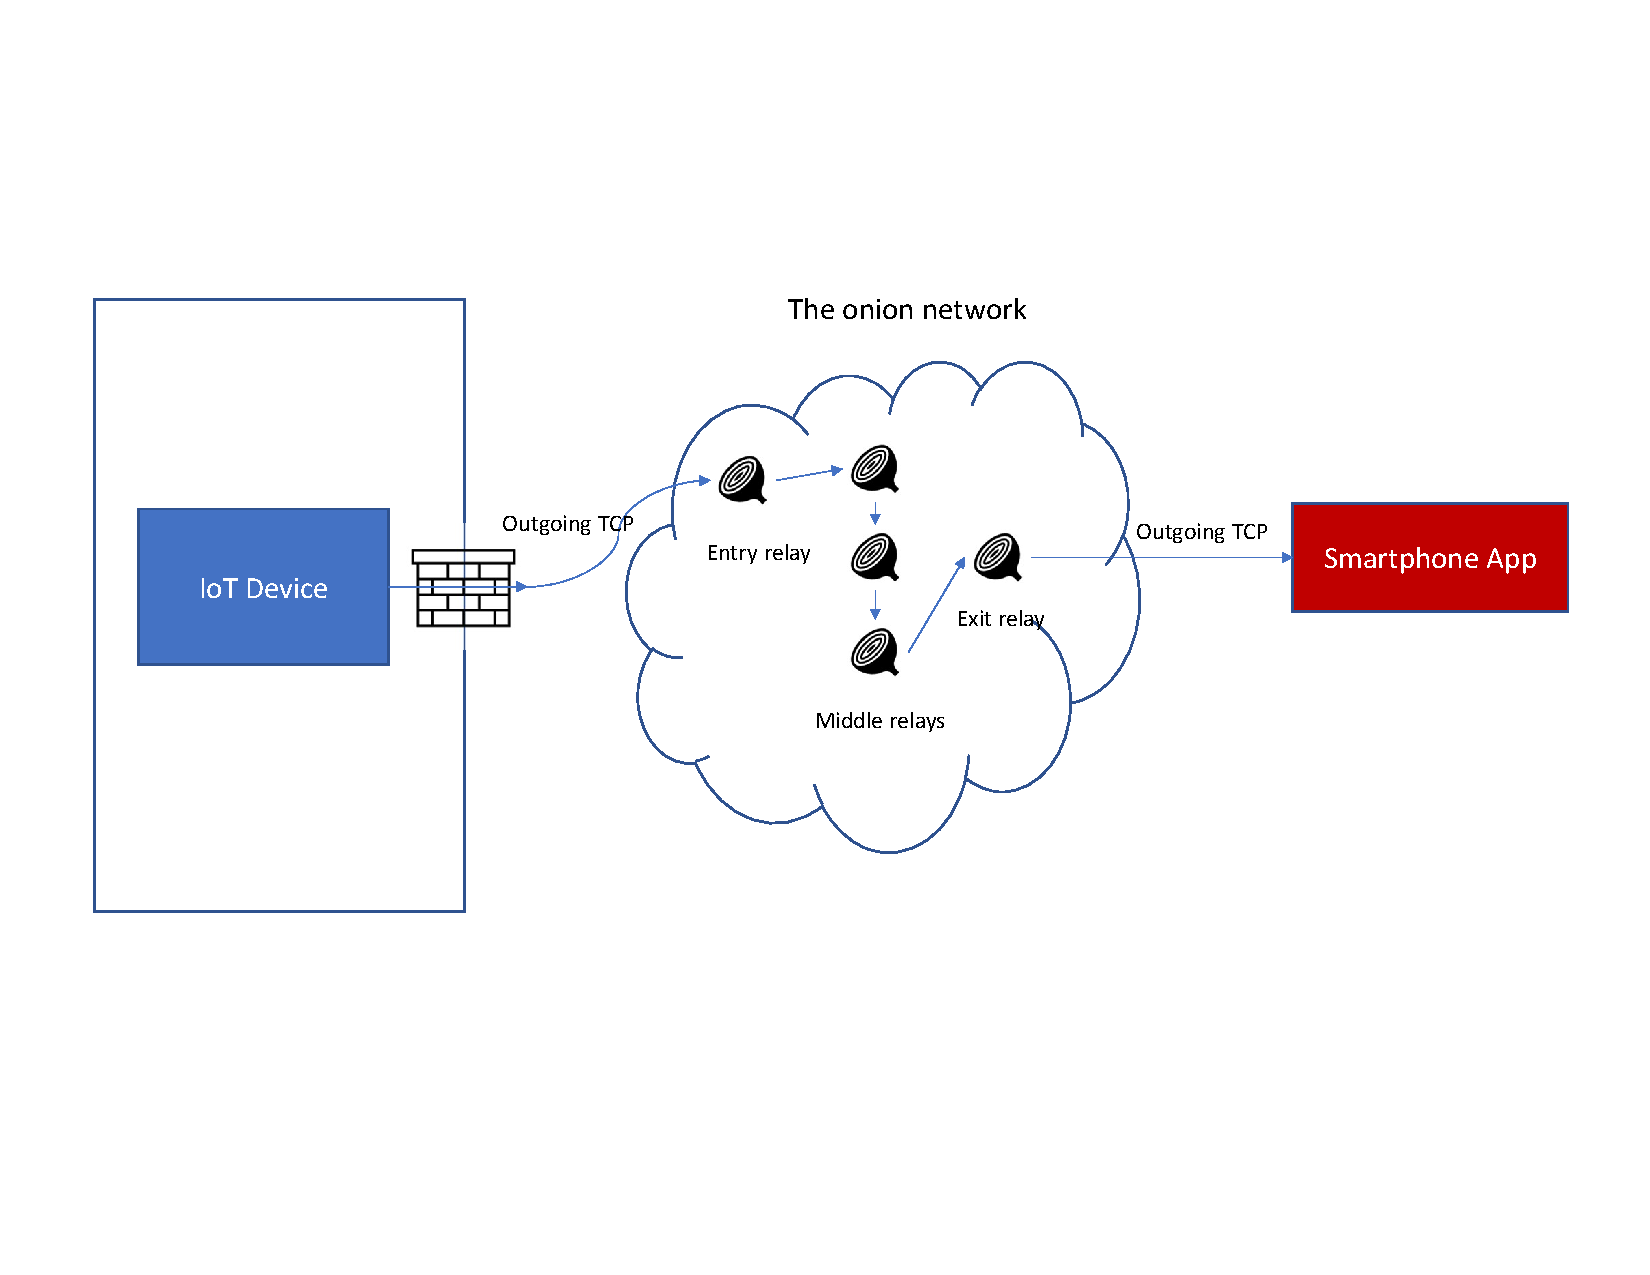
\includegraphics[width=\linewidth]{natpiercing.pdf}
	\caption{Network structure of onion-IoT}
	\label{fig:natpiercing}
\end{figure}
\chapter{A privacy-preserving framework for IoT devices}

In this chapter, we propose a privacy-preserving framework for generalized IoT devices by utilizing the Tor network. We propose communication and attacker models and state security and usability features of the framework.

\section{Communication models}

In this thesis, we consider only one communication model. In our model, the IoT devices interact with end-user devices (e.g., smartphones). The end-user devices have direct access and can remotely control the IoT device. 

It is worth mentioning that there exists another communication model for IoT systems. IoT devices sometimes need to communicate with each other to enable automatic workflows. However, we consider the first model to be primary in IoT systems and focus on it. We briefly discuss the IoT-to-IoT scenario in the discussion section. 

\section{Threat model}

Our analysis assumes an active network threat model where attackers are located both inside and outside the home network. The attackers may have capabilities similar or the same to an ISP.

Traditionally, IoT devices run globally searchable services\cite{antonakakis2017understanding}. Consequently, IoT devices are exposed to potential vulnerabilities and attacks. Attackers can exploit vulnerabilities through enumeration or DoS attacks to steal the data or take over the whole device.

Furthermore, mobile devices running paired service applications with home IoT devices usually access the Internet via untrusted networks, cellular networks, or free Wi-Fi hotspots. In such cases, on-path attackers can capture and inspect data packets, retrieve sensitive data or even locate and attack the communication's endpoint. 

In the following, we discuss potential attackers, their capabilities, and our system's security guarantees.
\subsection{Actors and capabilities}
We consider the following two types of adversaries:

\textbf{In-network adversaries} are adversaries who have access to the users' home network. Such adversaries may eavesdrop and identify traffic from particular devices in the user's home, including the doorbell device and router.


\textbf{Out of network but on-path adversaries} are adversaries located outside the user's home network (and have no access to it). Such adversaries cannot differentiate between devices in the network but can eavesdrop, analyze, and modify the user’s traffic in aggregate. 

Furthermore, the adversary can obtain and analyze IoT devices and client devices. They may inspect programs and source code and use their copy of client apps to access the user's device. Also, they may have access to the system's adapted push notification service, which means they can eavesdrop, modify the packets or send packets to the user's phone at his will.
\subsection{Security Guarantees}

\begin{itemize}
	\item \textbf{Strong authentication}: The device should only be accessible to authorized clients. \textit{Out-of-network adversaries} should not have access to the data (including the history of usage and data captures by the sensor) regardless of measurements they take.
	\item \textbf{Anonymity on both sides}: The communication between the client and home IoT device should be behind Tor. \textit{Out-of-network adversaries} should  get identical information (including IP address and physical address) of neither the client nor IoT device.
	\item \textbf{End-to-end security}: The traffic between the client and home IoT devices should be end-to-end encrypted. Neither \textit{In-network adversaries} nor \textit{Out-of-network adversaries} 
	\item \textbf{Attack resistance}: The attacks surface against the IoT devices should be small (e.g., resists DoS attacks)
\end{itemize}

\section{Feature}
In addition to the security guarantees, the system should have a few usability features:

\begin{itemize}
	\item \textbf{Direct access from end-user devices.} The system should be directly accessible from an end-user device. The user should be able to control and retrieve data from the device remotely. 
	\item \textbf{NAT-piercing.}  For compatibility with typical home networks, the system should work on devices located behind firewalls or gateway routers and do not have a public IP address.
	\item \textbf{Decentralization.} The system should try to avoid all points of decentralization. The user should not register to third-party services or external websites to have the service running or retrieving data.
	\item \textbf{Real-time data transmission.} The system should let its user retrieve data instantly and send notifications to the end-user device whenever the sensor has something detected.
\end{itemize}



\section{Methodology}
To achieve the security guarantees described above, we make the approach to introducing the Tor network in the communication between home IoT devices and end-user devices. The Tor network, a common approach for achieving anonymity\cite{dingledine2004tor}, has the following features, which makes it a good choice for privacy-preserving systems:

\begin{itemize}
	\item Anonymous connection: Taking advantage of the onion network structure, Tor client users are kept anonymous. Traffic packets are sent across multiple volunteer-hosted nodes (called onion relays). Packets are altered at each of the nodes by either adding or removing one layer of encryption. The client establishes a circuit involving several onion relays to the destination. In a Tor circuit, each relay only knows 1) which relay it is sending data to and 2) which relay has sent it data. In such a structure, the client user is kept anonymous during data transmission. 
	\item Hiding service locations: In addition, onion services also keep the server (receiver) anonymous. By the nature of anonymity, it protects the server from denial-of-service (DoS) and physical attacks. As a side effect, onion services can run on devices that are behind a firewall or gateway router, and thus providing the feature of NAT-piercing. Given that most home networks are behind gateway routers and home IoT devices usually do not have a public IP address, such a side effect is very attractive for IoT devices.
\end{itemize}
\chapter{Case-study: A privacy-Preserving Video Doorbell}

In this chapter, we present a case study which focuses on the design and implementation of a specific type of IoT devices - an Internet-enabled video doorbell. We assume the communication model to be the user-to-IoT model, where the IoT device (video doorbell) is located in the user's home network and communicates with the end-user device (smartphone).

\section{System design}
In addition to the security guarantee described in the last chapter, video doorbell systems has some unique features. Here we present design of the specific system.

\subsection{Use case analysis}
We consider there should be four main use cases in the system:
\begin{itemize}
	\item \textbf{Registration.}The user should be able to register a mobile device to the doorbell. Only trusted devices can access the data and manage settings.
	\item \textbf{Video streaming.} The user with a registered device should be able to access video captured by the camera at any time he wishes.
	\item \textbf{Face detection and push notification.}Whenever a visitor shows in front of the camera and/or pressed the physical doorbell button, all users registered to the doorbell should receive a push notification message.
	\item \textbf{Setting management.} The user should be able to manage settings, including changing face detection threshold, recording voice to be played, removing trusted devices, etc.
\end{itemize}

\textit{Fig. \ref{fig:usecase}} shows the use case diagram of the system.

\begin{figure}
	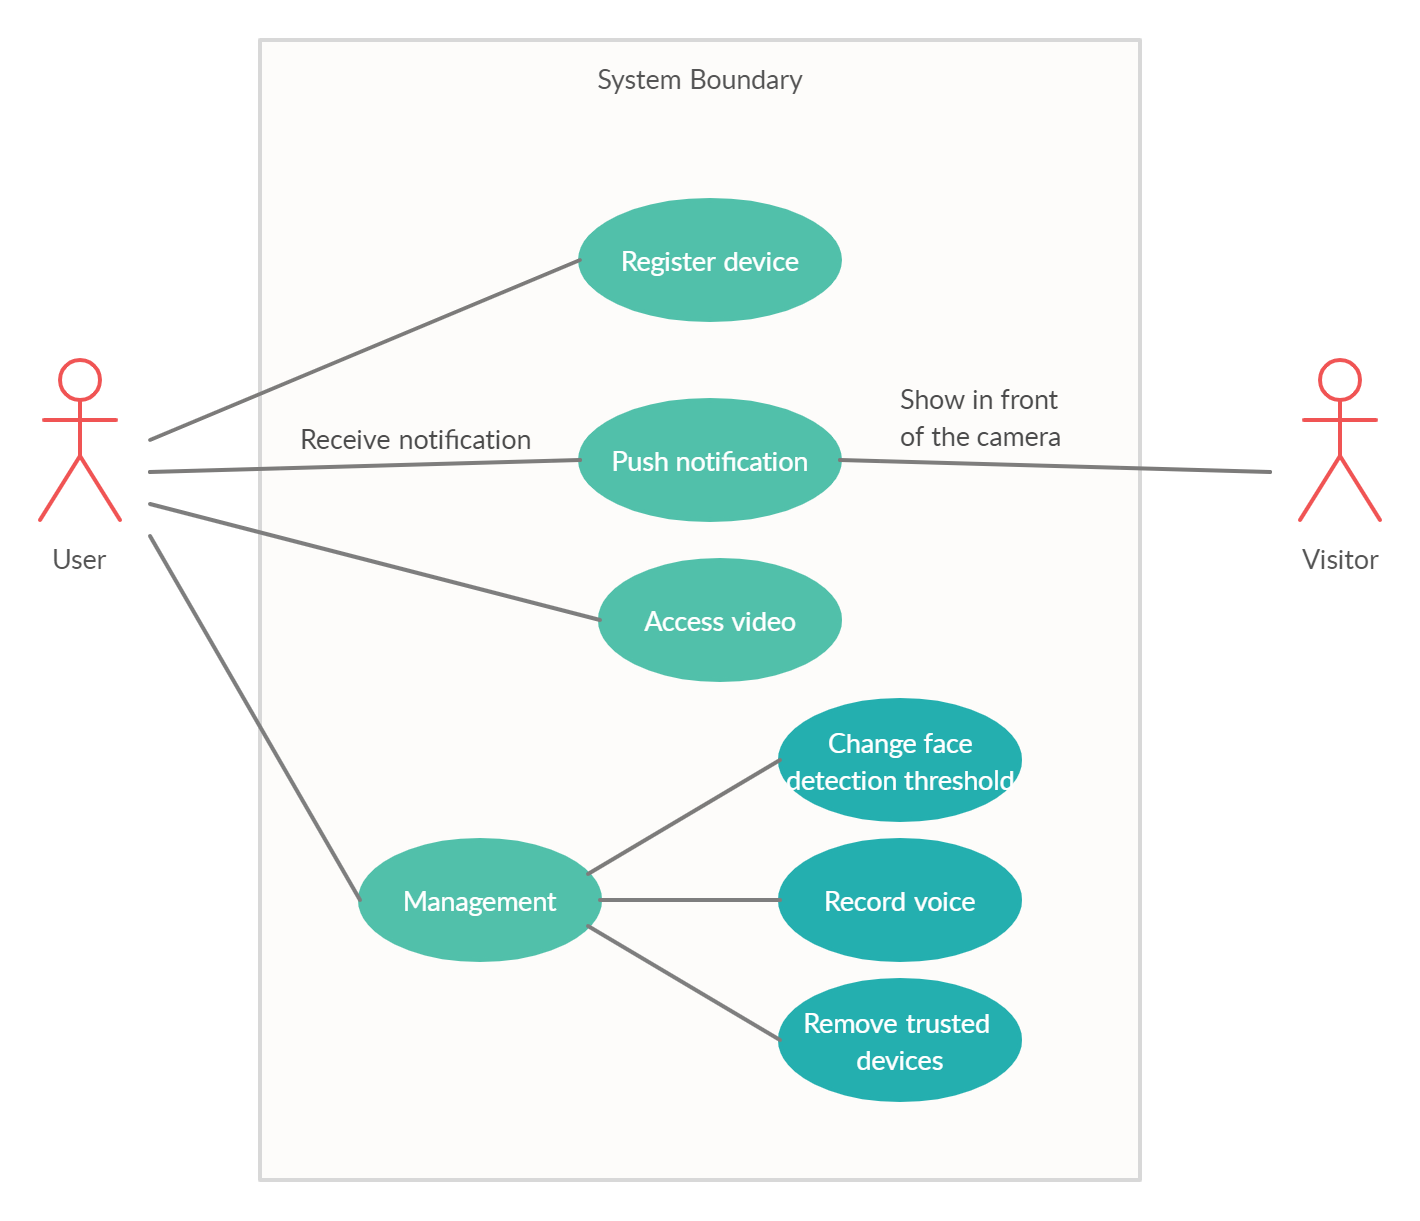
\includegraphics[width=\linewidth]{Use_case_diagram.png}
	\caption{}
	\label{fig:usecase}
\end{figure}

\subsection{Network architecture}
\textit{Fig. \ref{fig:architecture}} shows the network architecture of the system. Both the client and server are behind Tor for anonymity. In addition, we configure Tor on the doorbell side to use Snowflake \cite{snowflake} pluggable transport for obscuration.

\begin{figure}
	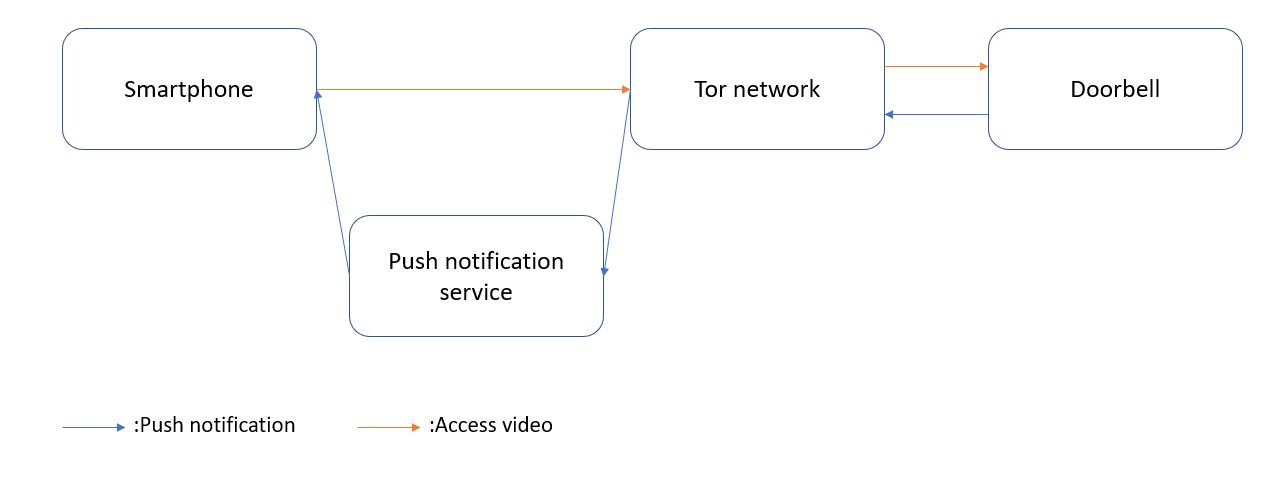
\includegraphics[width=\linewidth]{architecture.png}
	\caption{}
	\label{fig:architecture}
\end{figure}

\subsection{Flow structure}

\textbf{Registration.} The very first stage of using the system is the registration process. To have their devices registered on the doorbell, the users should first connect to the same wireless network with the doorbell. Then the app should allow the user to easily register (by searching the doorbell using mDNS). During the registration process, the app performs a key exchange with the doorbell and receives randomly generated credentials for user to set up in Tor (Orbot).

\textbf{Playing video and authentication.} As soon as the user presses the PLAY button in the app, it will work with Orbot and send a RTMP PLAY request to the video server running on the doorbell. The video server will then forward an authentication request (in the form of a HTTP GET request) to the authentication server (running on another port on the doorbell). The server should serve video to the user through Tor if the authentication succeeds (i.e. the app is registered and has not been revoked), and shut down the connection otherwise.
\textit{Fig. \ref{fig:playvideo}} shows the flow of playing video and authentication.

\textbf{Face detection, push notification and answering the door.} The doorbell constantly detects if there is a human face appearing in front of the camera. Whenever a visitor appears, the system should send a notification to the user's devices.

By clicking on the notification message on her phone, the user should be able to access the video immediately, and choose to play pre-recorded audio on the doorbell device to the visitor.
\textit{Fig. \ref{fig:push}} shows the flow of face detection, push notification and answering the door.

\begin{figure}
	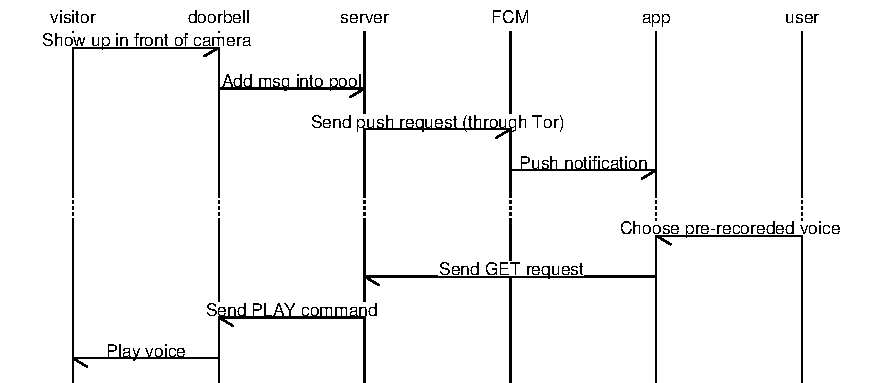
\includegraphics[width=\linewidth]{Sequence_diagram_push.pdf}
	\caption{}
	\label{fig:pushnotification}
\end{figure}
\begin{figure}
	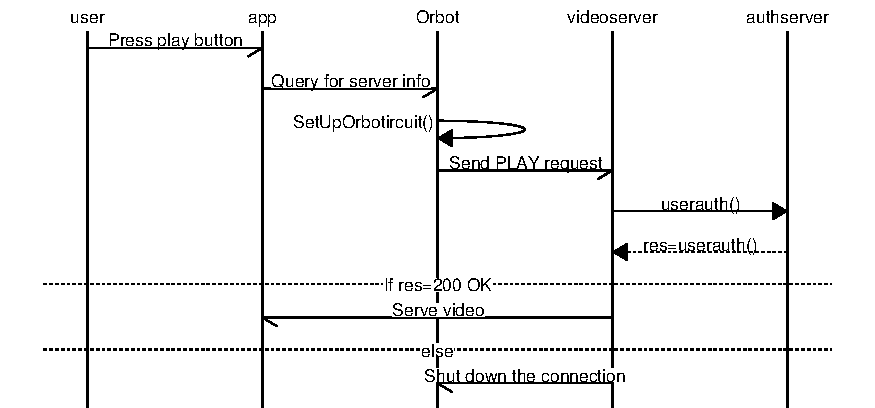
\includegraphics[width=\linewidth]{Sequence_diagram_playvideo.pdf}
	\caption{}
	\label{fig:playvideo}
\end{figure}
\begin{figure}
	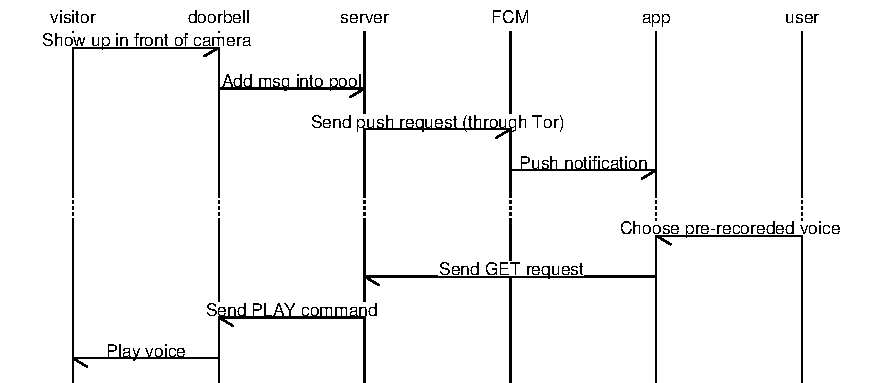
\includegraphics[width=\linewidth]{Sequence_diagram_push.pdf}
	\caption{}
	\label{fig:push}
\end{figure}

\section{Specs of the devices}
We configured a RaspberryPi 4 model B as the doorbell device. The RaspberryPi 4 has a built-in WiFi antenna, and we combined the device with a camera module and external sound card. The RaspberryPi ran the Raspbian Jessie OS, which is a version of Debian Linux optimized for the RaspberryPi platform.

The RaspberryPi 4 model is equipped with more than 2GB of RAM and a CPU with 1.5 GHz, which makes it more than enough for a typical home IoT device.

\section{Face detection}

For the face detection task, we use pre-trained CascadeClassifier. Cascade Classifiers based on Haar-like features was introduced in 2001 and still widely used in face detection \cite{sharifara2014general}. Pre-trained Cascade Classifiers have short execution time and small calculation load, which makes them a good choice for on-device calculations on IoT devices with low computational power.

In the actual implementation, we sample 6 frames per second, transform them into gray-scale images and feed them to the pre-trained classifiers. The detector is disabled for 5 seconds (which also matches the interval of push notification) after a successful detection to prevent abusing resources.

\section{Push notification}
To notify the user whenever a visitor is present in front of the camera, the system adapts Google's Firebase Messaging Service.

We designed two types of messages: \textbf{BELL} (sent when someone pushes the physical button of the doorbell device) and \textbf{DOOR} (sent when someone comes in front of the camera). The packet includes a message (including the type mentioned above), a timestamp and the user's instance token. The message and timestamp are encrypted using AES-256-GCM with pre-shared keys (which are shared in the registration process described later).

In order to prevent the third-party service provider from obtaining information by analyzing the timing information, we further cover the traffic using another message type \textbf{DUMMY} and send messages in a fixed interval of 5 seconds. The dummy packets have very similar structure with the normal ones, but has a different type to be recognized by the client app. By padding the dummy packets to the traffic, the system sends a packet every 5 second.






\section{Video streaming}
The doorbell device captures video using the RaspberryPi's camera module and audio through an external sound card. The video captured is encoded and served in flv format through HTTP. We chose to decode the videos in flv format because it is consistent among different operating systems and good for future enhancement of support on other platforms. 

Our system adapts two layers of authentication on top of video streaming. The first layer of authentication is the \textit{onion authentication}. Provided along with Tor, it requires the user to have certain credentials set up in their Tor (Orbot) client. The onion host refuses to connect if one do not have such settings, or have different settings. The second layer of authentication is the \textit{RTMP authentication}. In order to access the video, the user will have to add a couple of arguments in additional to their RTMP PLAY request. \textit{Fig. \ref{fig:url}} shows the components of the video serving url. In the url \textit{appname} and \textit{streamname} are Nginx settings and of the user's choice. \textit{usertoken} is a random number securely generated from the client app (upon first launch) and \textit{userpassword} is calculated by the following equation:

\[
userpassword = HMAC-SHA256(seed, usertoken)
\]

The server checks if \textit{all} credentials match, and shut down the connection if any are incorrect.

\begin{figure}
	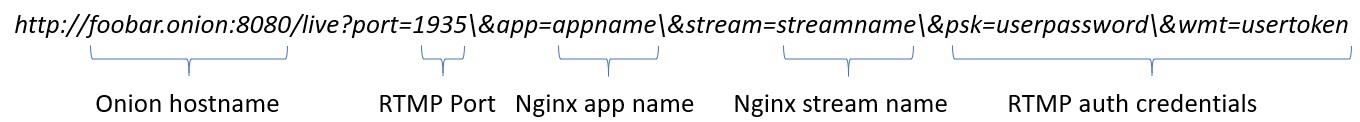
\includegraphics[width=\linewidth]{fig_url.jpg}
	\caption{}
	\label{fig:url}
\end{figure}



\section{Android App}
We implemented an Android App to pair with the video doorbell service. The app runs on the end-user device, and grant user direct access to the doorbell device and data. The app has the following primary functions:

\subsection{Registration} For registration, the client sends JSON-formatted data in a HTTP POST request to port 8080 of the server (running on the doorbell device). The server will then response with another JSON-formatted data, including the seed (randomly generated 16-bit integer) for calculating the secret keys, the onion hostname for accessing the video service and the onion authentication cookie. The app will then automatically send a configuration string (including the authentication cookie) required by Orbot to the user's clipboard, for her to easily set up the service.

\textit{Fig. \ref{fig:app_sc_main}} shows the main (registration) GUI of the app.


\subsection{Media player} The app has VLC player integrated for video streaming. Working with Orbot, the media player plays the video through the Tor network, which prevents adversaries from eavesdrop into the transmitted video.

\subsection{Management} The client sets up a webpage for the user to manipulate settings, including changing detection threshold, revoking authentications, recording voice, etc. The management page is only accessible in local network (that saying, the user device must be in the same wireless network with the doorbell device in order to manipulate settings) and require a password for accessing.

\textit{Fig. \ref{fig:app_sc_management}} shows the preference page, and \textit{Fig. \ref{fig:app_sc_token_revoke}} shows the token management (where user can revoke trusted devices) of the app.

\begin{figure}
	\begin{minipage}[t]{0.3\linewidth}
		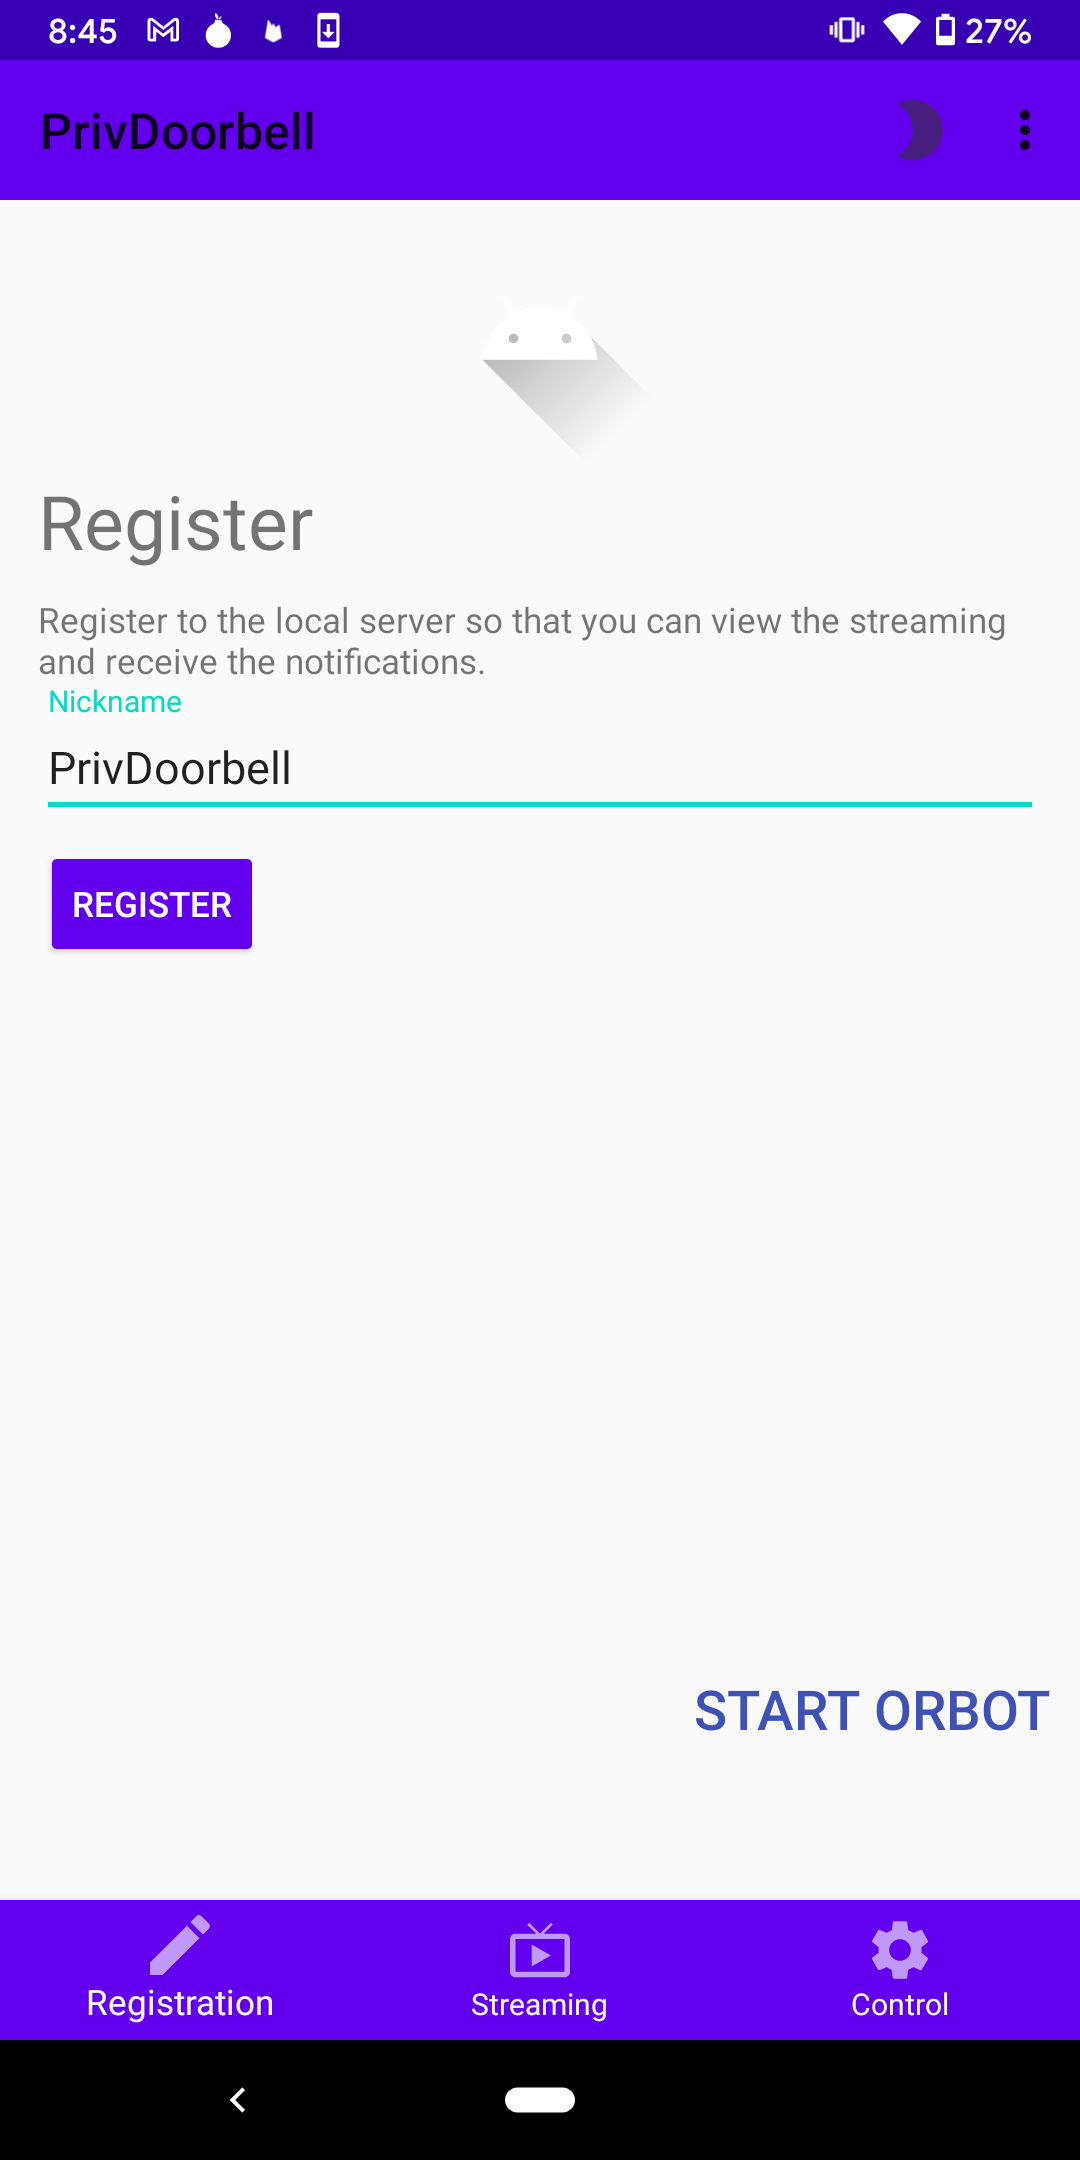
\includegraphics[width=0.5\linewidth]{app_sc_main.png}
		\caption{}
		\label{fig:app_sc_main}	
	\end{minipage}
	\begin{minipage}[t]{0.3\linewidth}
		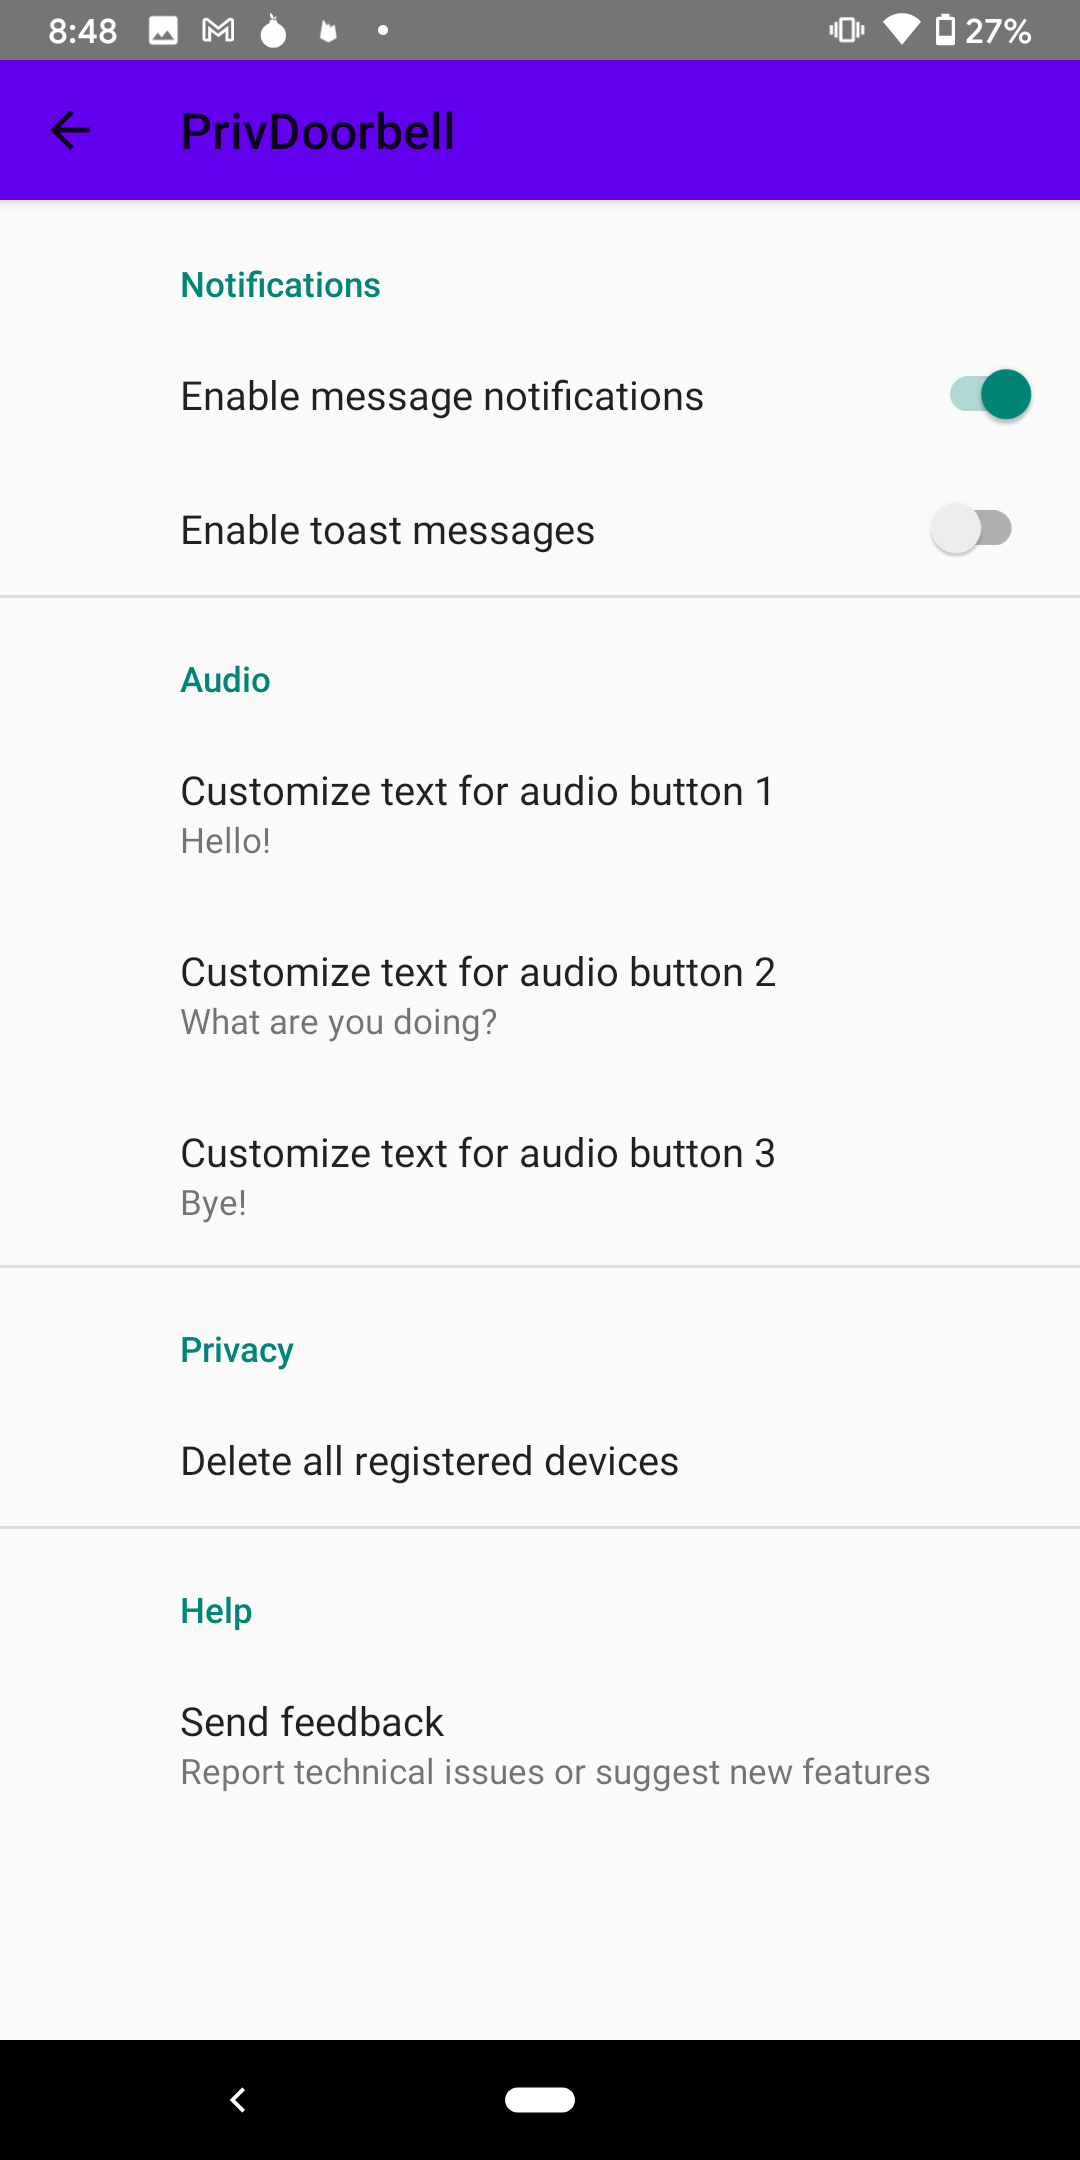
\includegraphics[width=0.5\linewidth]{app_sc_management.png}
		\caption{}
		\label{fig:app_sc_management}
	\end{minipage}
	\begin{minipage}[t]{0.3\linewidth}
		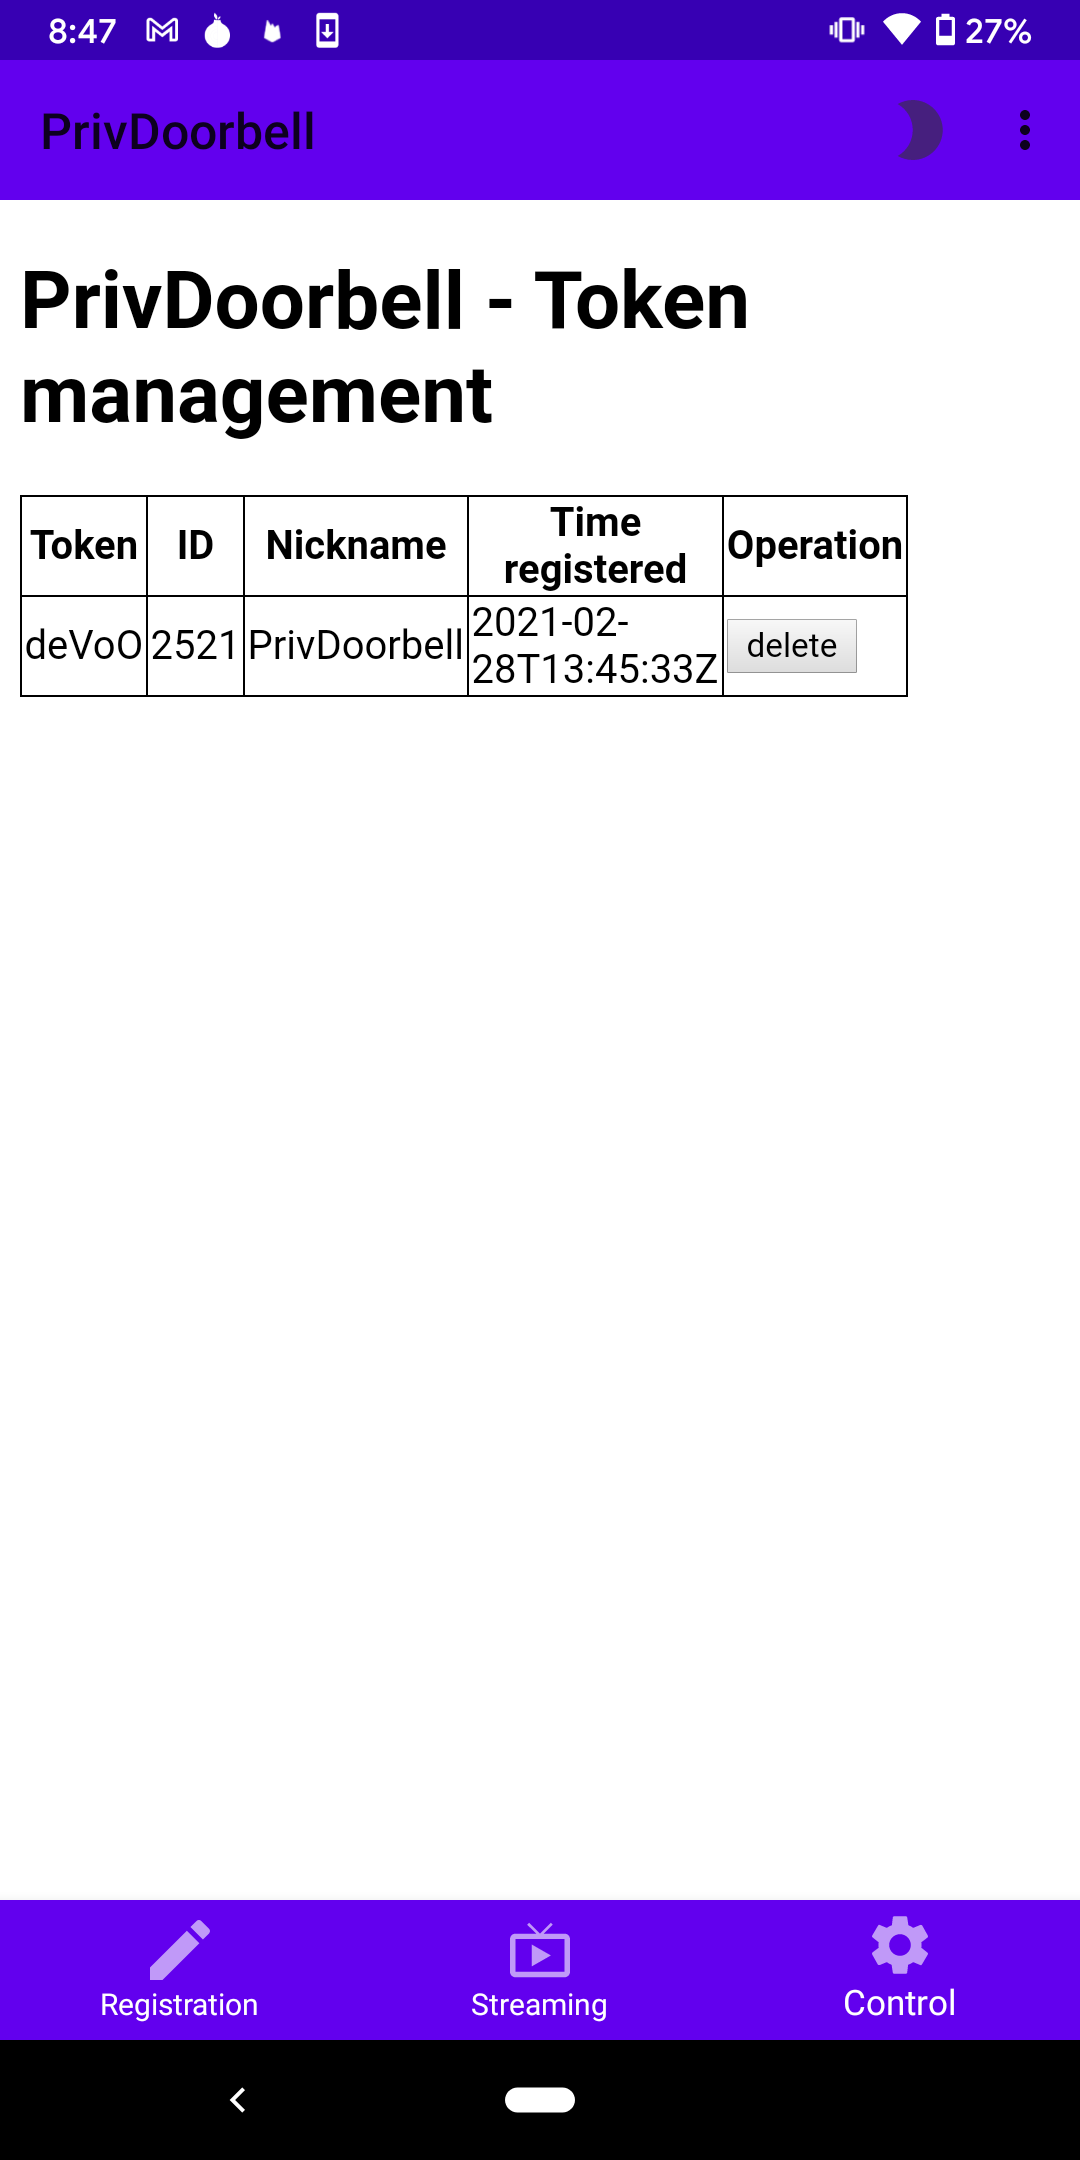
\includegraphics[width=0.5\linewidth]{app_sc_token_revoke.png}
		\caption{}
		\label{fig:app_sc_token_revoke}
	\end{minipage}	
\end{figure}


\section{Experimental study}
In this section, we would like to evaluate the performance of our system by analyzing the following factors:
\begin{itemize}
	\item Streaming latency
	\item Energy consumption
	\item Bandwidth
	\item Notification latency
	\item The cost of using Tor
\end{itemize}

A Google Pixel 3a XL is used as the client device.

\subsection{Streaming latency}
\label{subsec:streaming_latency}
We measure the latency of our system as the time difference between the user's pressing on the Play button and the first frame's appearing. \textit{Fig. \ref{fig:timeconsumption}} shows the time taken for 100 samples. We divide the time into four phrases.
\begin{itemize}
	\item Circuit: The \textit{Circuit} phrase is from when the app starts processing the user's request to when it receives the information of the server. In this phrase, the app queries the proxy (Orbot) about the onion url. Orbot will then try to establish a circuit connection the user device and the server. In practice, the time taken in this phrase varies, as sometimes there is an existing circuit. If Tor has to create a new circuit, this phrase typically takes a few more seconds. In average, this phrase takes 2.355 seconds with a standard derivation of 3.07 seconds.
	\item Transmission: The \textit{Transmission} phrase is from when the app sends request to the server to when the app hears back from the server. As we are using RTMP authentication, the server should return a HTTP answer code 200 if the client provides correct credentials. The video transmission will begin immediately after the HTTP response. In average, this phrase takes 0.599 seconds with a standard derivation of 0.089 seconds.
	\item Preparation: The \textit{Preparation} phrase is from when the app receives HTTP answer from the server to when it starts filling the buffer. In this phrase, the media player initializes its components and gets ready for playing the video. In average, this phrase takes 3.878 seconds with a standard derivation of 0.715 seconds.
	\item Buffering: The \textit{Buffering} phrase is when the app fills in its buffer. In this phrase, the media player fill a few frames into the buffer (of a programmed size) for the decoder to decode. The decoder will do the work in milliseconds, and thus we can consider the video being played immediately after this phrase. In average, this phrase takes 0.046 seconds with a standard derivation of 0.006 seconds.
\end{itemize}

\begin{figure}
	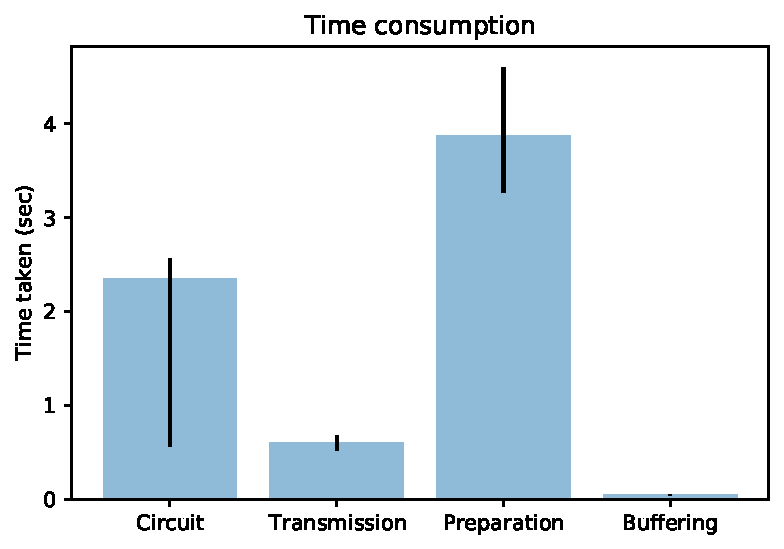
\includegraphics[width=\linewidth]{plot1.pdf}
	\caption{}
	\label{fig:timeconsumption}
\end{figure}

\begin{figure}
	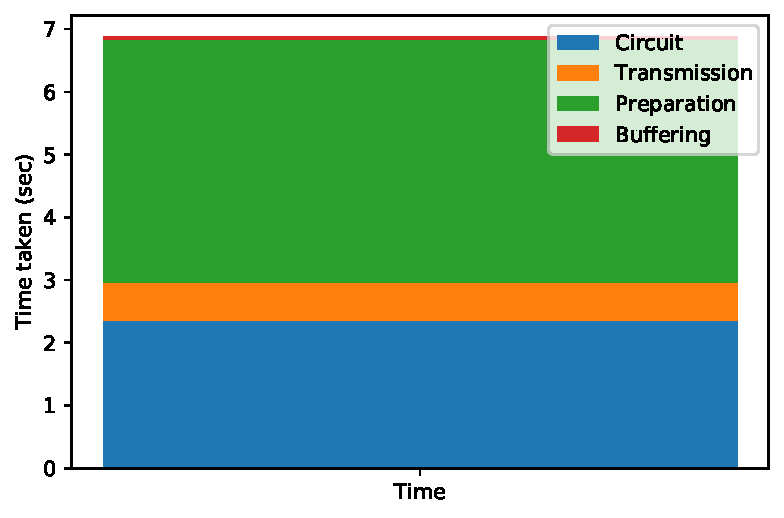
\includegraphics[width=\linewidth]{plot2.pdf}
	\caption{}
	\label{fig:timepercentage}
\end{figure}

In average, the whole process takes 6.867 seconds with a standard derivation of 3.141 seconds. \textit{Fig. \ref{fig:timepercentage}} shows how much time each phrase takes.


\subsection{Energy consumption}
We evaluate the battery consumption of our app using the system measured data. The app consumes 6\% of the device's battery after actively running in background for 6 days, 11 hours and 50 minutes (83.83 hours). The device has a battery size of 3700 mAh, and therefore the app roughly consumes 2.65 mAh for every hour running. We consider it reasonable for an app which receives and pushes real-time notifications.

\subsection{Bandwidth}
The outgoing traffic from the doorbell devices is 71 kb/s by average, after the video is compressed and encoded. For comparison, the raw video has the size of 410 kb/s.

\subsection{Video and audio quality}
The system supports videos up to 1024x768/6fps and audio with sample rate of 44.1kHz.

\subsection{Notification latency}
\label{subsec:notification_latency}
We measure the notification latency by measuring the time difference from when the message is sent to Firebase Messaging server from the doorbell to when the message is received on the client app. The average latency of 250 consecutive samples is 0.478 second. Fig. \cite{fig:notificationlatency_wTor} shows the CDF (cumulative distribution function) vs. latency (in second) diagram.

\subsection{The cost of using Tor}
Finally, we would like to measure the cost of using Tor. By its nature, Tor adds latency to the system and we would like to know the exact impact. We measure the following time and compare the difference:

\begin{itemize}
	\item Streaming latency
	\item Notification latency
\end{itemize}

\begin{figure}
	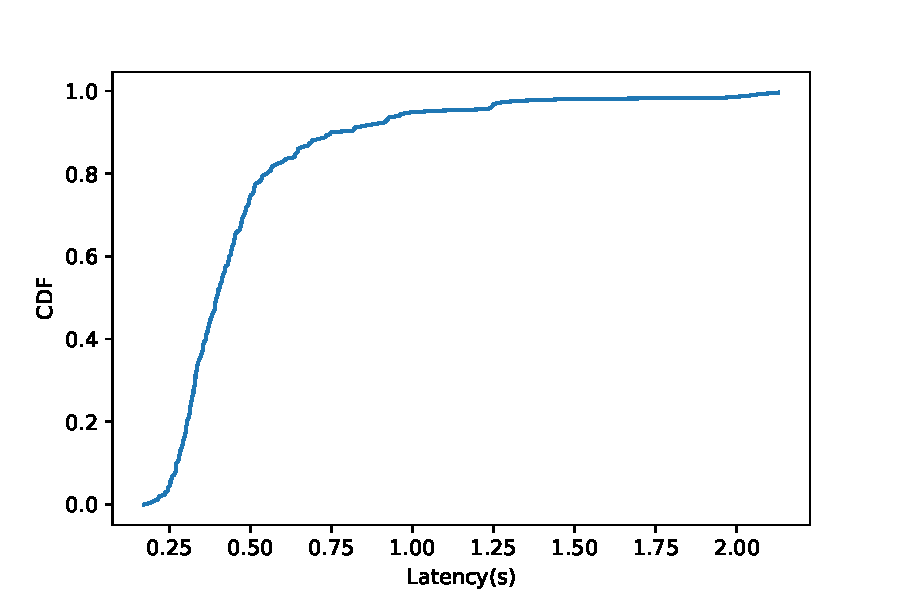
\includegraphics[width=\linewidth]{notification_latency_withTor.pdf}
	\caption{}
	\label{fig:notificationlatency_wTor}
\end{figure}

\paragraph{Streaming latency} 

We described the streaming latency of our system in \ref{subsec:streaming_latency}. For a simple comparison, launching the streaming takes 2.240 second on average.

\paragraph{Notification latency}

As we described in \ref{subsec:notification_latency}, the latency of push notification with Tor is 0.478 second on average. We further conduct experiment where Tor is not in the middle. \textit{Fig. \ref{fig:notificationlatency_wTor_vs_vanilla}} shows the difference of the service with Tor ("with-Tor") between that without Tor ("vanilla"). The dotted green line stands for the latency of vanilla service, and the blue full line stands for the latency of with-Tor service. The median of with-Tor service is roughly twice as the median of vanilla service.

\begin{figure}
	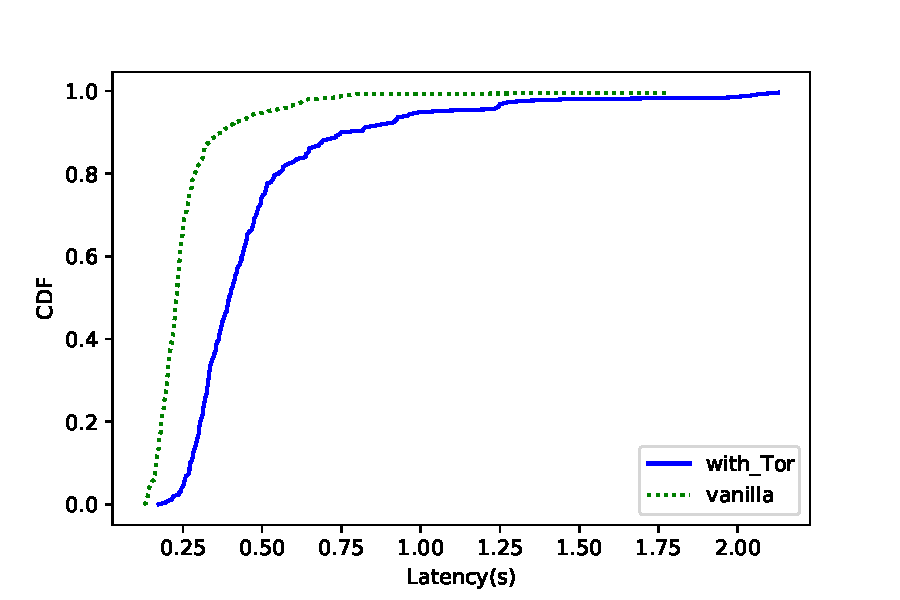
\includegraphics[width=\linewidth]{plot_push_tor_vs_vanilla.pdf}
	\caption{}
	\label{fig:notificationlatency_wTor_vs_vanilla}
\end{figure}
\chapter{Discussion and Open Questions}

\section{Traffic cover}
\label{sec:traffic_cover}
In the case study, we covered the traffic of push notifications by padding dummy packets and sending packets constantly (every 5 second). While constant padding is  a safe countermeasure against traffic analysis, the scheme may consume much more power than necessary since the interval of people visiting and thus non-cover message is usually far larger than 5 seconds. 

Prior research has proposed efficient ways of padding traffic. Perhaps most notably, Juarez \textit{et al.} \cite{juarez2016toward} proposed an adaptive padding algorithm and proved its effectiveness against traffic analysis. We consider it possible to adapt a similar algorithm in our system as a possible future enhancement.

\section{Decentralized push notification}
\label{sec:decentralized_push}
Ideally, our system would like to avoid all points of centralization and push notification is especially challenging since such alerting service are highly centralized. It is nearly impossible to push a notification with out using \textit{APNS (Apple Push Notification Service)} on an iOS device. It is somewhat easier on Android devices as Google permits the use of third-party push notification services. Unfortunately, most Android push notification services are designed to be 1-to-many systems (that is, one app developer pushes to many user devices), which makes it a bit difficult for private IoT devices to utilize such service.

In our case study, we used Firebase Cloud Messaging (formerly known as Google Cloud Messaging) as the push notification service provider. FCM is also designed as 1-to-many, and requires credentials for message senders. Therefore, in order to get a private channel for their own message, the users will have to register their own API key, include the key and compile the APK themselves. We consider the inconvenience a shortcoming of our system.

It is worth mentioning that implementing a private channel for push notifications is possible. A naive solution would be keeping a TCP socket open over Tor to receive notifications. Kollmann \textit{et al.} \cite{kollmann2017cost} discussed about the possibility and cost of push notifications using Tor, and pointed out that such solution is feasible but would consume more resource than most commercial push notification services.

For a proof-of-concept, we also implemented an experimental option for users to adapt such way of push notifications. In particular, we constructed our own push notification service for Android in which all communication occurs over the Tor network. Although we still reply on centralization (i.e., the push notification server), the use of Tor obfuscates clients' (the doorbells' and Android devices') locations, and prevents the centralized service from associating particular smartphones with doorbells. Further, it prevents the centralized server from easily enumerating the number of devices. We believe that such a privacy-preserving push notification is valuable for a number of uses outside of our IoT doorbell proof-of-concept. Experiments show that keeping the connection active for 4 hours consumes about 2\% of the device's battery. While the option is not ready for practical use (as there have been some unimplemented system-level issues, e.g. handling messages when the device is unavailable or the app has exited), it shows the possibility to deploy a fully decentralized push notification service with our system. We consider the full implementation to be one of the future enhancements.

\section{Storage}
In our proof-of-concept implementation, we did not add in the capability to store user videos. The videos are immediately discarded after being served. We consider it unsafe to store all the videos locally, as an adversary could physically steal or destroy the device. However, video doorbell users usually want to see what happened a few minutes or even a few days ago.

Most commercial video doorbells have applied the solution that they stored the video in their cloud server (and charge the users service fees). In this setting, the user's privacy completely depends on how the provider handles their information.

Another solution would be taking advantage of distributed storage. It is possible for users to form a distributed storage network, taking advantage of Distributed Hash Table \cite{stoica2001chord}. Thanks to DHT's property of being fault tolerant, it makes saving user data among all system users possible. There have been several approaches to apply DHT in IoT devices \cite{fabian2014privacy} \cite{paganelli2012dht}.

A practical problem with our system adapting distributed storage would be the size of data. Unlike most other IoT devices, video doorbells need to store and transmit large chunks of data (i.e. videos), which makes it difficult to implement in terms of fault tolerance.


\section{IoT devices in untrusted network}
In this thesis, we consider the home IoT device to be located in a trusted network (i.e. the home network). However, there are scenarios in which such devices will also be located in untrusted networks, for example the user is carrying the device while traveling. In such cases, additional attack surfaces and vulnerabilities are introduced as attackers can easily identify the IoT devices, analyze and manipulate the traffic. While such scenarios are not studied in this thesis, we consider it possible to adapt our solution with some additional security measurements. 

\section{IoT-to-IoT communication}
There is another communication model where IoT devices communicate with each other. This usually happens when a user has multiple home IoT devices and enables automatic workflows. While such a communication model is not covered in this thesis, it is possible to extend our solution so that each IoT device hosts its own onion service.
\chapter{Conclusion}
This thesis explores the challenge of designing privacy-preserving systems for home IoT devices. It reviews currently available home IoT devices, their privacy threats and the need for a privacy-preserving framework.

This thesis next proposes a privacy-preserving framework for generalized home IoT devices by combining Tor with IoT systems. We present different attacker models, security guarantees and usability features of such framework.

Then, it presents a case study which focuses on the detailed design and implementation of a specific type of home IoT systems - an Internet-enabled doorbell. We proposed the system design and implemented the system on a RaspberryPi computer. We also did experiments and analysis to argue the implemented system's usability.

Finally, we discuss  open questions that are not covered in this thesis, including better traffic cover mechanisms, completely decentralized push notification service, distributed storage and different communication models.


\appendices  % Indicates that appendices follow.
% If there's only one, use \appendix instead.


\chapter{First Appendix}\label{app:first}

\chapter{Second Appendix}

%\bibliographystyle{plainnat}
%\bibliography{thesis}  % thesis.bib

\bibliographystyle{bibs/ACM-Reference-Format}
\bibliography{bibs/bibs}

\typeout{***}
\typeout{*** Note!}
\typeout{*** Because this document has a table of contents,}
\typeout{*** you must run LaTeX TWICE to get it to print correctly.}
\typeout{***}

\end{document}

